%  ╔═╗┌─┐┌┬┐┌─┐┌┐┌┌─┐┌─┐  ┌┬┐┌─┐  ╔╦╗┌─┐┬─┐┬┌─┌─┐┬  ┬
%  ║  ├─┤ ││├┤ │││├─┤└─┐   ││├┤   ║║║├─┤├┬┘├┴┐│ │└┐┌┘
%  ╚═╝┴ ┴─┴┘└─┘┘└┘┴ ┴└─┘  ─┴┘└─┘  ╩ ╩┴ ┴┴└─┴ ┴└─┘ └┘ 

\chapter{Caracterización de la variabilidad del valor de medición usando modelos de Markov}

En esta sección se explica el diseño e implementación del método propuesto para tener en cuenta la variabilidad del
nivel indicado en la pantalla del sonómetro bajo calibración en el resultado de medición, expresado como el valor de
medición junto con la incertidumbre expandida de medición.
En primer lugar, se describen las consideraciones previas que dan validez al método propuesto y se introduce el
algoritmo que resume la ejecución del método en una serie de pasos.
Luego, se presenta el fundamento teórico suficiente de los procesos estocásticos modelados con cadenas de Markov y se
describen brevemente los detalles de la implementación del método.
Finalmente, se muestra y discute un ejemplo de un valor de medición obtenido con el método implementado y su
correspondiente incertidumbre de medida tipo A\@.

\section*{Consideraciones previas}
\addcontentsline{toc}{section}{Consideraciones previas}
El nivel instantáneo ponderado en tiempo y en frecuencia definido en la ecuación~\eqref{eq:time_weighted_level} no es
un indicador representativo del nivel de sonidos cuya presión tiene bastante variabilidad, ya que es muy susceptible a
las variaciones instantáneas en la presión acústica.
Por lo que normalmente en mediciones acústicas se evalúa el nivel de sonido promediado en el tiempo o nivel de sonido
continuo equivalente, definido en la
\mbox{IEC 61672--1}~\citeyearpar{IEC_TC29_2013_1} como
%
\begin{equation}
    \label{eq:equivalent_level}
    L_{Xeq,T} = 10\log{\left(\frac{\frac{1}{t_1 - t_2}\,\int_{t_2}^{t_1} p_X^2\left(\xi\right)\,\mathrm{d}\xi}{p_0^2}\right)}.
\end{equation}
%
En que $t_1$ y $t_2$ son el instante de tiempo final e inicial de integración correspondientemente.
El nivel continuo equivalente es un indicador mucho más confiable, ya que se trata de un nivel constante que, durante
todo el tiempo de integración, tiene la misma energía acústica que la señal de presión con sus variaciones instantáneas.

Ahora, medir el nivel equivalente requiere una intervención manual del usuario para ajustar en el sonómetro el tiempo de
integración y ver el resultado final, por lo que este indicador no es el más adecuado para la automatización empleando
reconocimiento de imágenes.
No obstante, la \mbox{IEC 61672--3}~\citeyearpar{IEC_TC29_2013_3} permite seleccionar entre un nivel ponderado en el
tiempo o un nivel promediado en el tiempo, como valor de medición en cada punto de calibración.
Para no comprometer la automatización y obtener un resultado de medición válido y representativo de todas las posibles
variaciones que pueda tener el nivel instantáneo ponderado en el tiempo, se propone tener en cuenta todas las muestras
del nivel ponderado en el tiempo y luego, el nivel presente en la mayor cantidad de muestras viene a ser una estimación
apropiada del nivel promediado en el tiempo (esto en condiciones controladas, como es el caso en laboratorios de
calibración).
Este efecto se puede comprobar analizando las expresiones matemáticas de cada indicador.
En primer lugar, de la ecuación~\eqref{eq:time_weighted_level} se extrae que la presión acústica con ponderación
temporal, expresada como una función del tiempo es
%
\begin{equation}
    p_{XY}^2(t) = \frac{1}{\tau_{Y}}\,\int_{-\infty}^t p_X^2\left(\xi\right)\,
    e^{\nicefrac{-\left(t - \xi\right)}{\tau_Y}}\,\mathrm{d}\xi.
\end{equation}

Esta presión instantánea ponderada en el tiempo no es la misma de la ecuación~\eqref{eq:equivalent_level}.
Para calcular un nivel continuo equivalente con ponderación temporal y frecuencial se requiere modificar la
ecuación~\eqref{eq:equivalent_level} remplazando $p_X^2(\xi)$ por $p_{XY}^2(t)$; en efecto, queda
%
\begin{align}
    L_{XYeq,T} &= 10\log{\left(\frac{\frac{1}{t_1 - t_2}\,\int_{t_2}^{t_1} p_{XY}^2(t)\,\mathrm{d}t}{p_0^2}\right)}; \nonumber \\
    &= 10\log{\left(\frac{\frac{1}{\tau_Y\,\left(t_1 - t_2\right)}\,
    \int_{t_2}^{t_1} \int_{-\infty}^t p_X^2\left(\xi\right)\,
    e^{\nicefrac{-\left(t - \xi\right)}{\tau_Y}}\,\mathrm{d}\xi\,\mathrm{d}t}{p_0^2}\right)}. \label{eq:equivalent_time_weighted_level}
\end{align}

De la ecuación~\eqref{eq:equivalent_time_weighted_level} se puede concluir que cuanto más tiempo permanezca estable
una presión acústica instantánea ponderada en tiempo, el nivel equivalente más se acercará al correspondiente nivel
instantáneo ponderado en tiempo, pues tiene mayor efecto en el resultado de la integral.

\section*{Cadenas de Markov de tiempo discreto}
\addcontentsline{toc}{section}{Cadenas de Markov de tiempo discreto}

\subsection*{Matriz de probabilidades de transición}
\addcontentsline{toc}{subsection}{Matriz de probabilidades de transición}

Tomando como guía el libro de Dobrow~\citeyearpar{Dobrow2016} y el de Gubner~\citeyearpar{Gubner2006}, una cadena de
Markov es un proceso aleatorio con la propiedad particular de que, dados unos valores del proceso desde el tiempo cero
hasta el tiempo actual, la probabilidad condicional del valor del proceso en algún tiempo futuro depende solo del valor
actual, es decir, el futuro y el pasado son condicionalmente independientes dado el presente.
Analíticamente, una cadena de Markov es una secuencia de variables aleatorias $X_0, X_1, \dots$ que toman valores del
espacio discreto de estados $\mathcal{S}$ con la propiedad de que
%
\begin{equation}
    \label{eq:markov_chain}
    P\left(X_{n + 1} = j\,|\,X_0 = x_0, \dots, X_{n - 1}
    = x_{n - 1}, X_n = i\right) = P\left(X_{n + 1} = j\,|\,X_n = i\right),
\end{equation}
%
Para todo $x_0, \dots, x_{n - 1}, i, j \in \mathcal{S}$ y $n \ge 0$.
Normalmente, se asume que todas las cadenas de Markov son homogéneas, en las que la probabilidad no depende de $n$.

En la ecuación~\eqref{eq:markov_chain} las probabilidades solamente dependen de $i$ y $j$, por lo que estas se pueden
organizar de forma matricial en $\mathbf{P}$, cuya $ji$-ésima entrada es
$p_{ij} = P\left(X_{n + 1} = j\,|\,X_n = i\right)$, la probabilidad de transición de un estado a otro en un paso.
La matriz de transición es una matriz cuadrada de $k \times k$ para los $k$ estados en el espacio $\mathcal{S}$.

La matriz de transición o matriz estocástica debe cumplir que $p_{ij} \ge 0 \quad \forall\,i,j$ y que
%
\begin{equation*}
    \sum_j p_{ij} = \sum_j P\left(X_{n + 1} = j\,|\,X_n = i\right)
    = \sum_j \frac{P\left(X_{n + 1} = j, X_n = i\right)}{P\left(X_n = i\right)}
    = \frac{P\left(X_n = i\right)}{P\left(X_n = i\right)} = 1.
\end{equation*}
%
Lo que indica que las transiciones en las cadenas de Markov son exhaustivas.

Teniendo en cuenta este fundamento conceptual, para cada punto de calibración se conforma una matriz de transición en
la que cada nivel diferente indicado en pantalla es un estado en la cadena de Markov.

\subsection*{Distribución de probabilidad estacionaria}
\addcontentsline{toc}{subsection}{Distribución de probabilidad estacionaria}

Una vez se conforma una matriz con las probabilidades de transición se puede usar álgebra matricial para hacer cálculos
con las probabilidades.
Uno de los más elementales es el cálculo de las probabilidades de transición del estado $i$ al $j$ en $n \ge 1$ pasos,
es decir $p_{ij}^{(n)} = P\left(X_n = j \,|\,X_0 = i\right)$, la probabilidad de que en $n$ pasos el proceso visite el
estado $j$ dado que ahora está en el estado $i$.
Cuando $n = 1$ las probabilidades son las mismas de $\mathbf{P}$, pero cuando $n \ge 1$ las probabilidades de transición
son los $ij$-ésimos elementos de la potencia $n$ de $\mathbf{P}$, denotada como $\mathbf{P}^n$.

Es de especial interés conocer el comportamiento del sistema en el largo plazo, lo cual está caracterizado por las
potencias de mayor orden de $\mathbf{P}$.
En la medida en que $n$ incrementa, el proceso alcanza un comportamiento límite y las probabilidades de transición
convergen a una distribución de equilibrio, conocida como distribución límite, la cual no depende de la distribución de
probabilidad inicial de los estados.
Para una cadena de Markov la distribución límite es la distribución de probabilidad $\boldsymbol{\lambda}$ con la propiedad de
que para todo $i$ y $j$
%
\begin{equation}
    \lim_{n\to\infty} \mathbf{P}_{ij}^n = \lambda_{j}.
\end{equation}

Si una cadena de Markov tiene una distribución límite, entonces esta es única.
Se puede encontrar la distribución límite simplemente tomando las potencias de mayor orden hasta obtener una matriz
$\boldsymbol{\Lambda}$ en la cual todas las filas son iguales a $\boldsymbol{\lambda}$, o también se pueden encontrar soluciones
exactas de forma analítica y teórica.
Cabe mencionar que la distribución límite también puede ser interpretada como la proporción de tiempo que el proceso
visita cada estado en el largo plazo

Ahora, si se asigna la distribución límite como la distribución inicial de la cadena de Markov, luego se encuentran las
probabilidades marginales $\boldsymbol{\lambda}\,\mathbf{P}$, y el resultado es el mismo vector $\boldsymbol{\lambda}$, entonces
esta distribución límite es llamada distribución estacionaria.
Es decir, una distribución estacionaria es una distribución de probabilidad $\boldsymbol{\pi}$ que satisface
$\boldsymbol{\pi} = \boldsymbol{\pi}\,\mathbf{P}$, o lo que es igual
%
\begin{equation}
    \label{eq:stationary_distribution}
    \pi_j = \sum_i \pi_j\, \mathbf{P}_{ij}, \quad \forall\, j.
\end{equation}

Aunque la distribución límite y la estacionaria están relacionadas, una cadena de Markov puede tener más de una
distribución estacionaria o ninguna, y esta no necesariamente es la distribución límite.
Pero si la cadena tiene una distribución límite, entonces esa distribución es estacionaria.
Esto depende directamente de la topología de la cadena;
si la cadena es regular entonces su matriz de transición $\mathbf{P}$ es regular (todos los valores de alguna de sus
potencias son positivos), y la distribución límite es igual a la estacionaria.

Para encontrar la distribución estacionaria cuando la matriz es regular, la forma más directa es resolver el sistema
lineal de ecuaciones que resulta de combinar la ecuación~\eqref{eq:stationary_distribution} y la restricción
$\sum_i \boldsymbol{\pi}_i = 1$.
La ecuación~\eqref{eq:stationary_distribution} puede escribirse matricialmente como
$\boldsymbol{\pi}\,(\mathbf{P} - \mathbf{I}) = \mathbf{0}$, o, para operar con vectores columna, como
$\left(\mathbf{P}^\intercal - \mathbf{I}\right)\,\boldsymbol{\pi} = \mathbf{0}$.
Finalmente, se puede escribir el sistema de ecuaciones matricialmente como
%
\begin{align}
    \mathbf{A}\,\boldsymbol{\pi} &= \mathbf{b}; \\
    \left[\begin{matrix}
              \left(\mathbf{P}^\intercal - \mathbf{I}\right) \\ 1 \cdots 1
    \end{matrix}\right]\,\boldsymbol{\pi} &= \left[\begin{matrix}
                                                       0 \\ 0 \\ \vdots \\ 1
    \end{matrix}\right].
\end{align}

Para encontrar soluciones para $\boldsymbol{\pi}$ se resuelve la ecuación
\begin{equation}
    \label{eq:pi_linear_system}
    \left(\mathbf{A}^\intercal\,\mathbf{A}\right)\,\boldsymbol{\pi} = \mathbf{A}^\intercal\,\mathbf{b}.
\end{equation}

\subsection*{Valor esperado}
\addcontentsline{toc}{subsection}{Valor esperado}

En un sistema discreto, el valor esperado calculado a partir de la distribución estacionaria es
%
\begin{equation}
    \mathrm{E}[X] = \sum_n x_n\,\pi_n,
\end{equation}

\section*{Algoritmo para la creación del modelo de Markov}
\addcontentsline{toc}{section}{Algoritmo para la creación del modelo de Markov}
El método propuesto consiste en tomar cada uno de los niveles instantáneos obtenidos como un estado en una cadena de
Markov.
Esta cadena caracteriza los cambios de un nivel a otro, considerando la variabilidad del nivel instantáneo como un
proceso estocástico.
Luego, con la distribución de probabilidad estacionaria se estima el valor esperado en el largo plazo, que lógicamente
corresponde al estado (nivel instantáneo) con mayor probabilidad de ocurrir.
Las probabilidades de transición de un estado a otro se determinan a partir de una serie de muestras de niveles
instantáneos obtenidas durante un tiempo de $25$ segundos aproximadamente, y la cantidad de muestras depende del periodo
de actualización del nivel instantáneo en la pantalla del sonómetro.
Por tanto, el valor esperado calculado con la cadena de Markov será probablemente el nivel instantáneo que más muestras
tuvo y será el valor de medición.
Este es un proceso que se realiza en cada punto de calibración y se resume en el siguiente algoritmo.

\begin{algorithm}[H]
    \caption{Algoritmo para el cálculo del valor esperado usando cadenas de Markov.}
    \label{alg:markov_expected_value}
    \scriptsize
    \DontPrintSemicolon
    \SetKwData{frames}{frames}
    \SetKwInOut{Output}{output}
    \KwData{\frames $\leftarrow$ \text{Vídeo de $\qty{25}{\s}$ del nivel instantáneo indicado en pantalla.}}
    \Output{Valor esperado}
    \BlankLine
    \textbf{\hyperref[sec:downsampling]{Paso 1}:} Submuestrear y reconocer cuadros después del tiempo de estabilización.\;
    \textbf{\hyperref[sec:transition_matrix]{Paso 2}:} Conformar matriz de transición de estados.\;
    \textbf{\hyperref[sec:stationary_distribution]{Paso 3}:} Calcular distribución de probabilidad estacionaria.\;
    \textbf{\hyperref[sec:expected_value]{Paso 4}:} Calcular valor esperado.\;
\end{algorithm}

Las operaciones efectuadas en cada paso, se describen y se ilustran mediante un ejemplo tomado de una ejecución del
algoritmo en la prueba de ponderación frecuencial $Z$ con señales eléctricas a la frecuencia de $\qty{63}{\Hz}$.

\section*{Paso 1: Submuestreo y reconocimiento de cuadros después de la estabilización}
\addcontentsline{toc}{section}{Paso 1: Submuestreo y reconocimiento de cuadros después de la estabilización}
\label{sec:downsampling}

Como el nivel con ponderación temporal \emph{Fast}, que tiene una constante de tiempo $\tau_F = \qty{125}{\ms}$,
requiere un tiempo transitorio hasta que el nivel se estabilice después de enviar la señal eléctrica.
Se determinó experimentalmente un tiempo de $\qty{2}{\s}$.
Los cuadros obtenidos durante este tiempo de estabilización no se tienen en cuenta para la matriz de transición,
pero sí para determinar el cuadro cero con el que se sincroniza la actualización del nivel instantáneo en pantalla con
los cuadros del vídeo.

Para determinar el cuadro cero primero se efectúa el algoritmo~\ref{alg:image_recongnition} en los cuadros del tiempo
de estabilización.
Con el vector de los valores numéricos reconocidos se encuentra el índice del primer cambio detectado de valor.
Luego, a los cuadros después de ese índice se les hace un submuestreo según la relación entre la tasa de cuadros por
segundo de la cámara y la tasa de actualización de la pantalla del sonómetro.
Los cuadros que quedan corresponden al instante exacto en el que hay una nueva muestra en pantalla.
Sin embargo, dado que puede presentarse en la pantalla LCD un efecto de solapamiento entre la muestra anterior y la
nueva, que afecta negativamente el reconocimiento de imágenes, se determinó experimentalmente tomar $2$ cuadros después
del cuadro en el que ocurre el cambio, para permitir la estabilización de la pantalla.

\tikzmath{\x1 = -0.2; \x2 = 20;}
\begin{figure}[!h]
    \caption{Serie adquirida de cuadros de estabilización (naranja), de medición (negro) y submuestreados con
        corrimiento de dos posiciones (rojo)}
    \label{fig:frames_series}
    \centering
    \begin{tikzpicture}[inner sep=1pt, minimum height=1.8cm]
        \node[process, draw=orange, align=center] (frame0) at (0,0) {
\includegraphics[height=\x2pt]{5_MC_incertidumbre/Frames/frame(0)}\\[\x1em] idx: $0$\\[\x1em] \texttt{\small nan}};
        \node[process, draw=orange, align=center, right=0cm of frame0] (frame1) {
\includegraphics[height=\x2pt]{5_MC_incertidumbre/Frames/frame(1)}\\[\x1em] idx: $1$\\[\x1em] \texttt{\small nan}};
        \node[process, text=orange, minimum height=0.5cm, above=0cm of frame1] (tstab){$t_{\mathrm{stab}} = \qty{2}{s} \quad \longrightarrow$};
        \node[process, draw=orange, align=center, right=0cm of frame1] (frame2) {
\includegraphics[height=20pt]{5_MC_incertidumbre/Frames/frame(2)}\\[\x1em] idx: $2$\\[\x1em] \texttt{\small nan}};
        \node[process, right=0cm of frame2] (dots1) {$\cdots$};
        \node[process, draw=orange, align=center, right=0cm of dots1] (frame38) {
\includegraphics[height=\x2pt]{5_MC_incertidumbre/Frames/frame(38)}\\[\x1em] idx: $38$\\[\x1em] \texttt{\small nan}};
        \node[process, draw=blue, thick, align=center, right=0cm of frame38] (frame39) {
\includegraphics[height=\x2pt]{5_MC_incertidumbre/Frames/frame(39)}\\[\x1em] idx: $39$\\[\x1em] $32.6$};
        \node[process, text=blue, above=0cm of frame39, minimum height=0.5cm] (zeroframe) {cuadro cero};
        \node[process, draw=orange, align=center, right=0cm of frame39] (frame40) {
\includegraphics[height=\x2pt]{5_MC_incertidumbre/Frames/frame(40)}\\[\x1em] idx: $40$\\[\x1em] $32.6$};
        \node[process, draw=red, thick, align=center, right=0cm of frame40] (frame41) {
\includegraphics[height=\x2pt]{5_MC_incertidumbre/Frames/frame(41)}\\[\x1em] idx: $41$\\[\x1em] $32.6$};
        \node[process, draw=orange, align=center, below=0cm of frame0] (frame42) {
\includegraphics[height=\x2pt]{5_MC_incertidumbre/Frames/frame(42)}\\[\x1em] idx: $42$\\[\x1em] $32.6$};
        \node[process, draw=orange, align=center, right=0cm of frame42] (frame43) {
\includegraphics[height=\x2pt]{5_MC_incertidumbre/Frames/frame(43)}\\[\x1em] idx: $43$\\[\x1em] $32.6$};
        \node[process, draw=orange, align=center, right=0cm of frame43] (frame44) {
\includegraphics[height=\x2pt]{5_MC_incertidumbre/Frames/frame(44)}\\[\x1em] idx: $44$\\[\x1em] $32.6$};
        \node[process, draw=orange, align=center, right=0cm of frame44] (frame45) {
\includegraphics[height=\x2pt]{5_MC_incertidumbre/Frames/frame(45)}\\[\x1em] idx: $45$\\[\x1em] $32.6$};
        \node[process, draw=red, thick, align=center, right=0cm of frame45] (frame46) {
\includegraphics[height=\x2pt]{5_MC_incertidumbre/Frames/frame(46)}\\[\x1em] idx: $46$\\[\x1em] $32.6$};
        \node[process, draw=orange, align=center, right=0cm of frame46] (frame47) {
\includegraphics[height=\x2pt]{5_MC_incertidumbre/Frames/frame(47)}\\[\x1em] idx: $47$\\[\x1em] $32.6$};
        \node[process, draw=orange, align=center, right=0cm of frame47] (frame48) {
\includegraphics[height=\x2pt]{5_MC_incertidumbre/Frames/frame(48)}\\[\x1em] idx: $48$\\[\x1em] $32.6$};
        \node[process, draw=orange, align=center, below=0cm of frame42] (frame49) {
\includegraphics[height=\x2pt]{5_MC_incertidumbre/Frames/frame(49)}\\[\x1em] idx: $49$\\[\x1em] $33.2$};
        \node[process, draw=orange, align=center, right=0cm of frame49] (frame50) {
\includegraphics[height=\x2pt]{5_MC_incertidumbre/Frames/frame(50)}\\[\x1em] idx: $50$\\[\x1em] $33.2$};
        \node[process, draw=red, thick, align=center, right=0cm of frame50] (frame51) {
\includegraphics[height=\x2pt]{5_MC_incertidumbre/Frames/frame(51)}\\[\x1em] idx: $51$\\[\x1em] $33.2$};
        \node[process, right=0cm of frame51] (dots2) {$\cdots$};
        \node[process, draw=orange, align=center, right=0cm of dots2] (frame97) {
\includegraphics[height=\x2pt]{5_MC_incertidumbre/Frames/frame(97)}\\[\x1em] idx: $97$\\[\x1em] $33.2$};
        \node[process, draw=orange, align=center, right=0cm of frame97] (frame98) {
\includegraphics[height=\x2pt]{5_MC_incertidumbre/Frames/frame(98)}\\[\x1em] idx: $98$\\[\x1em] $33.3$};
        \node[process, draw=orange, align=center, right=0cm of frame98] (frame99) {
\includegraphics[height=\x2pt]{5_MC_incertidumbre/Frames/frame(99)}\\[\x1em] idx: $99$\\[\x1em] $33.3$};
        \node[process, draw=orange, align=center, right=0cm of frame99] (frame100) {
\includegraphics[height=\x2pt]{5_MC_incertidumbre/Frames/frame(100)}\\[\x1em] idx: $100$\\[\x1em] $33.3$};
        \node[process, below=0cm of frame50, minimum height=0.5cm] (tmeas) {$t_{\mathrm{meas}} = \qty{25}{s} \quad\longrightarrow$};
        \node[process, draw=red, thick, align=center, below=0.5cm of frame49] (frame101) {
\includegraphics[height=\x2pt]{5_MC_incertidumbre/Frames/frame(101)}\\[\x1em] idx: $101$\\[\x1em] $33.3$};
        \node[process, draw, align=center, right=0cm of frame101] (frame102) {
\includegraphics[height=\x2pt]{5_MC_incertidumbre/Frames/frame(102)}\\[\x1em] idx: $102$\\[\x1em] $-$};
        \node[process, draw, align=center, right=0cm of frame102] (frame103) {
\includegraphics[height=\x2pt]{5_MC_incertidumbre/Frames/frame(103)}\\[\x1em] idx: $103$\\[\x1em] $-$};
        \node[process, draw, align=center, right=0cm of frame103] (frame104) {
\includegraphics[height=\x2pt]{5_MC_incertidumbre/Frames/frame(104)}\\[\x1em] idx: $104$\\[\x1em] $-$};
        \node[process, draw, align=center, right=0cm of frame104] (frame105) {
\includegraphics[height=\x2pt]{5_MC_incertidumbre/Frames/frame(105)}\\[\x1em] idx: $105$\\[\x1em] $-$};
        \node[process, draw=red, thick, align=center, right=0cm of frame105] (frame106) {
\includegraphics[height=\x2pt]{5_MC_incertidumbre/Frames/frame(106)}\\[\x1em] idx: $106$\\[\x1em] $33.3$};
        \node[process, draw, align=center, right=0cm of frame106] (frame107) {
\includegraphics[height=\x2pt]{5_MC_incertidumbre/Frames/frame(107)}\\[\x1em] idx: $107$\\[\x1em] $-$};
        \node[process, right=0cm of frame107] (dots3) {$\cdots$};
        \node[process, draw=red, thick, align=center, below=0cm of frame101] (frame111) {
\includegraphics[height=\x2pt]{5_MC_incertidumbre/Frames/frame(111)}\\[\x1em] idx: $111$\\[\x1em] $33.2$};
        \node[process, draw, align=center, right=0cm of frame111] (frame112) {
\includegraphics[height=\x2pt]{5_MC_incertidumbre/Frames/frame(112)}\\[\x1em] idx: $112$\\[\x1em] $-$};
        \node[process, right=0cm of frame112] (dots4) {$\cdots$};
        \node[process, draw=red, thick, align=center, right=0cm of dots4] (frame116) {
\includegraphics[height=\x2pt]{5_MC_incertidumbre/Frames/frame(116)}\\[\x1em] idx: $116$\\[\x1em] $33.2$};
        \node[process, right=0cm of frame116] (dots5) {$\cdots$};
        \node[process, draw=red, thick, align=center, right=0cm of dots5] (frame121) {
\includegraphics[height=\x2pt]{5_MC_incertidumbre/Frames/frame(121)}\\[\x1em] idx: $121$\\[\x1em] $33.1$};
        \node[process, right=0cm of frame121] (dots6) {$\cdots$};
        \node[process, right=0cm of dots6] (dots7) {$\cdots$};
        \node[process, draw=red, thick, align=center, right=0cm of dots7] (frame161) {
\includegraphics[height=\x2pt]{5_MC_incertidumbre/Frames/frame(161)}\\[\x1em] idx: $161$\\[\x1em] $33.2$};
        \node[process, right=0cm of frame161] (dots8) {$\cdots$};
        \node[process, right=0cm of dots8] (dots9) {$\cdots$};
    \end{tikzpicture}
    \caption*{\footnotesize Fuente: Elaboración propia.}
\end{figure}

En seguida, en el nuevo vector de cuadros submuestreado se busca el índice del cuadro inmediatamente después al tiempo
de estabilización, que corresponde al producto del tiempo de estabilización y la tasa de actualización de la pantalla
del sonómetro.
Finalmente, se efectúa el reconocimiento de los cuadros submuestreados a partir del índice del cuadro de estabilización
con el algoritmo~\ref{alg:image_recongnition}.
El vector de valores numéricos reconocidos es el arreglo de muestras a partir del cual se conforma la matriz de
transición de estados en el \hyperref[sec:transition_matrix]{paso 2}.

\begin{figure}[!h]
    \caption{Cuadro capturado con solapamiento en el dígito decimal entre el número $2$ y el $3$.}
    \label{fig:wrong_frame}
    \centering
    
\includegraphics[height=2cm]{5_MC_incertidumbre/Frames/wrong_frame}
    \caption*{\footnotesize Fuente: Elaboración propia.}
\end{figure}
%
Si en este punto aún resultara que el clasificador entregue un valor no numérico debido a un solapamiento como el de
la figura~\ref{fig:wrong_frame}, el valor no numérico es tomado como atípico y se elimina de la serie de muestras.

La figura~\ref{fig:frames_series} ilustra el proceso del paso 1 y en la siguiente figura se grafica el arreglo de
valores numéricos reconocidos.
%
\begin{figure}[!h]
    \caption{Serie de muestras de valores numéricos reconocidos.}
    \label{fig:recognized_samples}
    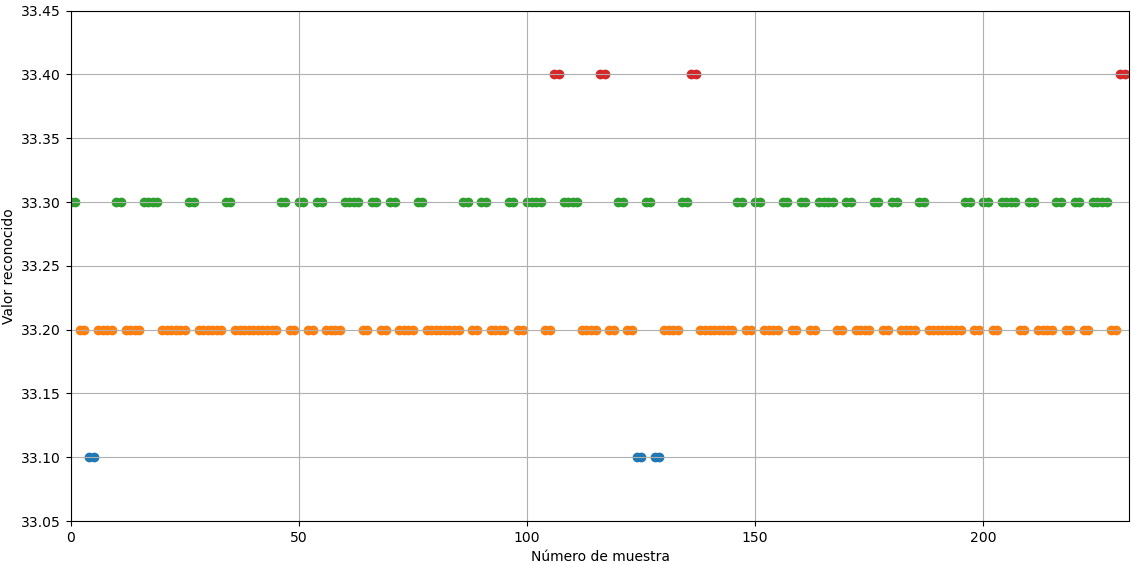
\includegraphics[width=\textwidth]{5_MC_incertidumbre/recognizedSamples}
    \caption*{\footnotesize Fuente: Elaboración propia.}
\end{figure}
\vfill

\section*{Paso 2: Conformar matriz de transición de estados}
\addcontentsline{toc}{section}{Paso 2: Conformar matriz de transición de estados}
\label{sec:transition_matrix}

\begin{code}
    \caption{Método estático para la construcción de una matriz de transición de estados a partir de una serie de muestras dada.}
    \label{code:build_transition_matrix}
    \centering
    \begin{minted}{python}
@staticmethod
def build_transition_matrix(samples: np.ndarray) -> np.ndarray:
    """
    Method for construction of the states transition matrix from a sequence of samples
    :param samples: A numpy one dimensional ndarray with the sequence of samples.
    :return: A numpy array that represents the transition matrix of the Markov model.
    """
    states = np.unique(samples)  # Remove repeated samples
    P = pd.DataFrame(data=np.zeros((states.shape[0], states.shape[0])), index=states, columns=states)  # Empty P
    for i in range(1, samples.shape[0]):  # Counts transitions from state to state
        P.loc[samples[i - 1], samples[i]] += 1
    P = P.div(P.sum(axis=1), axis=0)  # Computes probabilities
    return P
    \end{minted}
\end{code}
\begin{figure}[!h]
    \caption{Grafo de estados y probabilidades de transición que representa la matriz de transición~\eqref{eq:eg_transition_matrix}.}
    \label{fig:eg_automata}
    \centering
    \begin{tikzpicture}[thick,shorten >=1pt,node distance=6cm,on grid,auto]
        \node[state](q1){$\qty{33.1}{\dB}$};
        \node[state](q2)[below=of q1]{$\qty{33.2}{\dB}$};
        \node[state](q3)[right=of q1]{$\qty{33.3}{\dB}$};
        \node[state](q4)[below=of q3]{$\qty{33.4}{\dB}$};
        \draw[->, stealth-]
        (q1) edge [loop left] node {$\num{0.500}$} ()
        edge [bend right, swap] node {$\num{0.015}$} (q2)
        edge [swap] node {$\num{0.012}$} (q3)
        (q2) edge [loop left] node {$\num{0.712}$} ()
        edge [swap, pos=0.6] node {$\num{0.333}$} (q1)
        edge [bend right] node {$\num{0.395}$} (q3)
        edge [bend right, swap] node {$\num{0.286}$} (q4)
        (q3) edge [loop right] node {$\num{0.581}$} ()
        edge [bend right, swap] node {$\num{0.167}$} (q1)
        edge [bend right] node {$\num{0.250}$} (q2)
        edge [swap, pos=0.6] node {$\num{0.143}$} (q4)
        (q4) edge [loop right] node {$\num{0.571}$} ()
        edge [swap] node {$\num{0.023}$} (q2)
        edge [bend right, swap] node {$\num{0.012}$} (q3);
    \end{tikzpicture}
    \caption*{\footnotesize Fuente propia.}
\end{figure}

Para conformar la matriz de transición se escribió el método estático del código~\ref{code:build_transition_matrix}.
Una vez implementado correctamente en el desarrollo previo de la aplicación, se obtuvieron los resultados esperados.
Para el ejemplo ilustrado en el \hyperref[sec:downsampling]{paso 1}, la matriz de transición obtenida se presenta a
continuación.
Y el grafo correspondiente se representa en la figura~\ref{fig:eg_automata}.

\begin{equation}
    \label{eq:eg_transition_matrix}
    \mathbf{P} = \kbordermatrix{
        & \mathbf{\num{33,1}} & \mathbf{\num{33.2}} & \mathbf{\num{33.3}} & \mathbf{\num{33.4}} \\
        \mathbf{\num{33.1}} & \num{0.500} & \num{0.333} & \num{0.167} & \num{0.000} \\
        \mathbf{\num{33.2}} & \num{0.015} & \num{0.712} & \num{0.250} & \num{0.023} \\
        \mathbf{\num{33.3}} & \num{0.012} & \num{0.395} & \num{0.581} & \num{0.012} \\
        \mathbf{\num{33.4}} & \num{0.000} & \num{0.286} & \num{0.143} & \num{0.571} \\
    }.
\end{equation}

\section*{Paso 3: Calcular distribución de probabilidad estacionaria}
\addcontentsline{toc}{section}{Paso 3: Calcular distribución de probabilidad estacionaria}
\label{sec:stationary_distribution}

\begin{code}
    \caption{Método estático para el cálculo de la distribución límite de una cadena de Markov dada una matriz de transición.}
    \label{code:limit_dist}
    \centering
    \begin{minted}{python}
def limit_dist(P: np.ndarray) -> float:
    """
    Method to calculate the limit distribution with linear algebra solution using a given transition matrix P if
    the given matrix is a regular matrix, else, the calculation is performed with the high matrix powers of the
    transition matrix.
    :param P: The numpy array that represents de transition matrix.
    :return: The stationary distribution as a float number.
    """
    for n in range(2, 1001):
        if np.all(np.linalg.matrix_power(P, n) > 0):  # Check if it is a regular transition matrix
            # The matrix is regular, so limiting distribution exists and is the unique stationary distribution
            A = np.append(np.transpose(P) - np.identity(P.shape[0]), np.ones((1, P.shape[0])),
                          axis=0)  # Augmented A
            b = np.zeros((A.shape[0], 1))
            b[-1] = 1  # Augmented b
            PI = np.linalg.solve(np.transpose(A).dot(A), np.transpose(A).dot(b))  # Stationary distribution
            break
    else:
        PI = np.linalg.matrix_power(P, 1000)

    return PI
    \end{minted}
\end{code}

Para calcular la distribución límite dada una matriz de transición $\mathbf{P}$ se escribió
el método estático del código~\ref{code:limit_dist}.
Siguiendo con el ejemplo, al resolver el sistema lineal con el código implementado, la distribución estacionaria es
\begin{equation*}
    \boldsymbol{\pi} = \kbordermatrix{
        & \mathbf{\num{33.1}} &  \mathbf{\num{33.2}} &  \mathbf{\num{33.3}} & \mathbf{\num{33.4}} \\
        & \num{0.026} & \num{0.570} & \num{0.364} & \num{0.040}
    }.
\end{equation*}

\section*{Paso 4: Calcular valor esperado}
\addcontentsline{toc}{section}{Paso 4: Calcular valor esperado}
\label{sec:expected_value}

El valor esperado se obtiene directamente con
\mintinline{python}{expected_value = np.round(np.sum(np.array(P.index) * PI.T), 1)}.
Para el ejemplo, el valor esperado, redondeado a la misma cantidad de dígitos decimales de la precisión del sonómetro,
es $\qty{33.2}{\dB}$.

\section*{Evaluación tipo A de la incertidumbre típica}
\addcontentsline{toc}{section}{Evaluación tipo A de la incertidumbre típica}

De a cuerdo con la guía para la expresión de la incertidumbre de medida~\citep{ISO_TAG4_2008}, los valores de las
observaciones individuales $q_k$ difieren en razón de las variaciones aleatorias de las magnitudes de influencia o de
efectos aleatorios.
La varianza experimental de dichas $n$ observaciones está dada por:
%
\begin{equation}
    s^2\left( q_k \right) = \frac{1}{n - 1}\, \sum_{j = 1}^{n} \left( q_j - \bar{q} \right)^2,
\end{equation}
%
Que, junto con su raíz cuadrada positiva $s\left( q_k \right)$ (denominada desviación típica experimental), representan
la variabilidad de los valores $q_k$, es decir, su dispersion al rededor del valor esperado $\bar{q}$.
Luego, la mejor estimación de la varianza experimental de la media $\sigma^2\left( \bar{q} \right) = \sigma^2 / n$ es
%
\begin{equation}
    \label{eq:experimental_mean_variance}
    s^2\left( \bar{q} \right) = \frac{s^2\left( q_k \right)}{n},
\end{equation}
Que, junto con desviación típica experimental de la media $s\left( \bar{q} \right) = \sqrt{s^2\left( \bar{q} \right)}$
pueden ser utilizadas como medida de la incertidumbre de $\bar{q}$.

En concreto, en un modelo matemático de un mesurando $y$, para una magnitud de entrada $X_i$ obtenida a partir de $n$
observaciones repetidas e independientes $X_{i,k}$, la incertidumbre típica $u\left( x_i \right)$ de su estimación
$x_i = \bar{X}_i$ es $u\left( x_i \right) = s\left( \bar{X}_i \right)$, con $s^2\left( \bar{X}_i \right)$ calculada con
la ecuación~\eqref{eq:experimental_mean_variance}.
Esta incertidumbre típica $u\left( x_i \right)$ es llamada \emph{incertidumbre típica tipo A}.

El número de observaciones $n$ debe ser lo suficientemente grande para garantizar que $s^2\left( \bar{q} \right)$
proporcione una estimación fiable de la varianza $\sigma^2\left( \bar{q} \right)$.
La aplicación desarrollada permite cumplir esta consideración, puesto que en un tiempo de $\qty{25}{\s}$, con un periodo
de actualización de pantalla típico de $\qty{100}{\ms}$, se capturan $250$ muestras.
Ahora, en un cálculo posterior, cuando se determinan intervalos de confianza para la incertidumbre expandida, se debe
tomar en cuenta la diferencia entre $\sigma^2\left( \bar{q} \right)$ y $s\left( \bar{q} \right)$, ya que en muchos casos
puede ser que la distribución de probabilidad del mesurando (en este caso equivale a la distribución estacionaria) sea
muy distinta de una distribución normal.

La estimación de la incertidumbre típica tipo A puede hacerse rápidamente con la instrucción
\mintinline{python}{samples.std() / math.sqrt(samples.shape[0])}.
Para las muestras del ejemplo anterior se obtiene $s\left( \bar{q} \right) \approx \qty{0.004}{\dB}$.